\documentclass{article}
\usepackage{graphicx} % Required for inserting images
\usepackage[margin=1in]{geometry}
\usepackage{url}
\usepackage{hyperref}

\usepackage{float}
\usepackage{amsmath}
\usepackage{amssymb}

\usepackage{import}

\usepackage[calc]{datetime2}
\usepackage{pgfgantt}
\usepackage{datenumber}

\usepackage{pdflscape}

\title{CS310 Progress Report: Evaluating the Performance of Blink Detection on DeepFakes Injected With Adversarial Noise}
\author{Joel Coulon, 2204489}
\date{}

\begin{document}

\maketitle

\section{Project Introduction}

A DeepFake refers a video of an individual is digitally altered or created by an Artificial Intelligence (AI). These are often generated using Generative Adversarial Network (GANs) models and are trained via the adversarial of two models: one attempting to generate a realistic image, the other attempting to detect the inaccuracies. These two then train each other until the original model can generate videos that are deemed realistic by the detector.\\

Initially, these models were fairly obvious to detect, even for humans, for example see Figure \ref{fig:earlyexample}. Various features, such as temporal inconsistencies, feature irregularities, and inconsistencies in lighting produced by GANs were all tell-tale signs of DeepFaked imagery. However, over time, GANs have developed resulting in DeepFakes now being almost impossible to tell apart from genuine videos by humans.

\begin{figure}[H]
    \centering
    \fbox{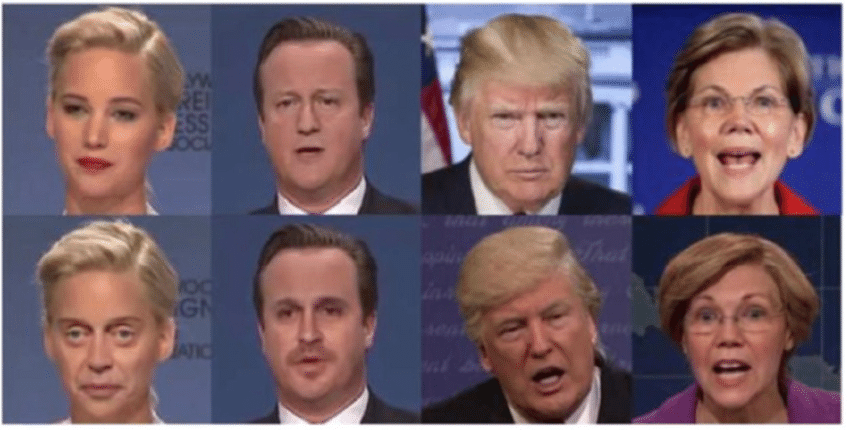
\includegraphics[width=0.5\linewidth]{images/Examples-of-original-and-deepfake-videos.png}}
    \caption{An early of example of DeepFakes with original images on the top, faked images on the bottom\cite{earlydeepfakeimage}}
    \label{fig:earlyexample}
\end{figure}

Due to their difficulty to be accurately identified by humans, DeepFakes soon became a popular way to spread misinformation by faking an individual's likeness. For example, DeepFakes were used by a variety of sources to promote political parties in the 2021 Lebanese elections\cite{misinformation}. The other primary use of DeepFakes is pornography with an estimated 98\% of DeepFakes being porn\cite{pornography}, including the first main-stream DeepFake in 2017 of actress Gal Gadot\cite{misinformation}.\\

Ever since the creation of DeepFakes there has been efforts to detect them. Original DeepFake detection methods relied on pixel analysis and visual artifacts present in early DeepFakes\cite{yu2021survey}. However through a combination of improvement in generation techniques and adversarial noise attacks\cite{huang2020fakeretouch}\cite{pertubations}, these original methods are proving increasingly ineffective.\\

One method proposed to tackle modern DeepFakes is blink detection. Blinking is a subconscious act for humans and falls into a predictable patterns. DeepFakes are notoriously bad at simulating blinking, either by not blinking at all or blinking in unnatural intervals. Thus methods have been used to leverage these temporal inconsistencies to detect DeepFakes with a high degree of accuracy\cite{blinking-pattern}.\\

So far, the resilience of blink-detection to adversarial noise has not been studied. It seems likely that due to this method relying on identification of features rather than individual pixels, it seems likely that adversarial noise would not affect the detection of a DeepFake in any meaningful way. This project aims to verify whether this assumption is true or not.

\section{Literature Review} \label{sec:literature-review}

This project combines two thoroughly-research topics (Blink-based DeepFake detection and Adversarial noise injection) which have had extensive research on both of them.

\subsection{Blink Detection}
\subsubsection{DeepVision}

DeepVision\cite{blinking-pattern} is a model that takes into account the time, activity, gender and age of the individual in a video to determine whether a video is DeepFaked or not by comparing their blink patterns to a database of known ``good" blink frequencies\\

The pre-process stage of the model involves categorising the video based on 4 landmarks. The landmarks are: gender, age (in 6 sub-categories varying from \textless 20 to 65+), activity (dynamic or static), and time (am/pm). The frequency of a human varies based on all these features\cite{varying-blink}, and therefore they believe all of these factors need to be taken into account for an accurate detection.\\

To actually detect a blink, two algorithms are used. The first is an algorithm called Fast-HyperFace\cite{ranjan2017hyperface} which is used to detect the landmarks of the face, pose, and gender of the individual in a video. The key landmarks from this are then extracted to then aid in the performance of the second model: Eye-Aspect Ration (EAR). EAR uses 6 points to calculate the absolute area of the horizontal versus the vertical axis to determine if a blink has occurred\cite{EAR}.
\begin{equation}
    EAR=\frac{||p_2-p_6||+||p_3-p_5||}{2||p_1-p_4||}
\end{equation}
The average of the left eye ($EAR_l$) and the right ($EAR_r$) can then be taken to get the mean eye ration ($EAR_i$)
\begin{equation}
    EAR_i = \frac{EAR_l + EAR_r}{2}
\end{equation}
\begin{figure}[H]
    \centering
    \fbox{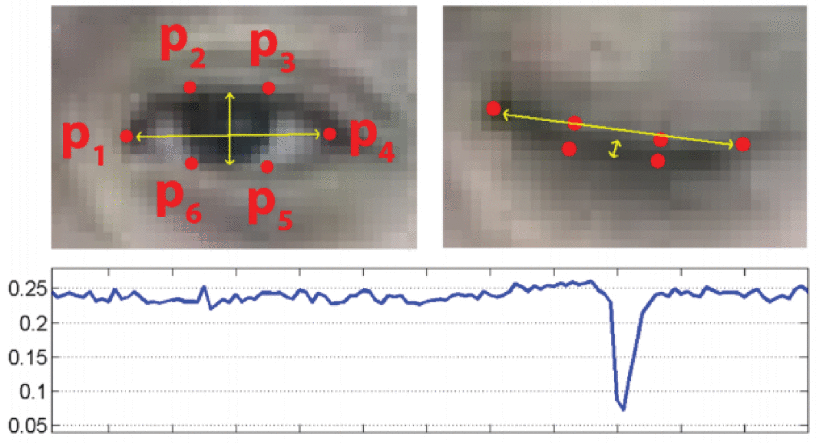
\includegraphics[width=0.5\linewidth]{images/EAR.png}}
    \caption{The EAR algorithm at work with eye landmarks $p_{1-6}$ labelled and a graph representing EAR (y-axis) over time (x-axis)}
    \label{fig:EAR}
\end{figure}

A blink is defined as when $EAR_i$ drops below a certain threshold for multiple consecutive frames. Data such as when the blink occurred in time, the period of blink, and frequency are all extracted and fed into the next stage.\\

This data is then compared with data from a pre-existing database of valid blinks derived from the Eye Blinking Prediction dataset from Kaggle\cite{eyeblinkprediction}. The factors mentioned above are all compared to see how similar they are to valid blinks in authentic videos and if it is within a certain threshold the video is deemed real. The paper does not mention this threshold. \\

DeepVision achieves an overall accuracy of 87.5\%\cite{blinking-pattern}.

\subsubsection{Ictu Oculi}

Ictu Oculi is a secondary method for blink detection, but rather than relying on an existing database for comparison, uses a trained neural network\cite{ictuoculi}.\\

An initial pre-processing step is done to identify the facial landmarks of the image and distort and crop it so that the face is: in the centre of the image; rotated such tat eyes form a horizontal line; and scaled to a similar size across the length of the video.\\

Once pre-processing is complete, the cropped video is sent to a Long-term Recurrent Convolution Neural Network (LRCN). This is three-stage neural network as shown in Figure \ref{fig:LRCN}. 

\begin{figure}[H]
    \centering
    \fbox{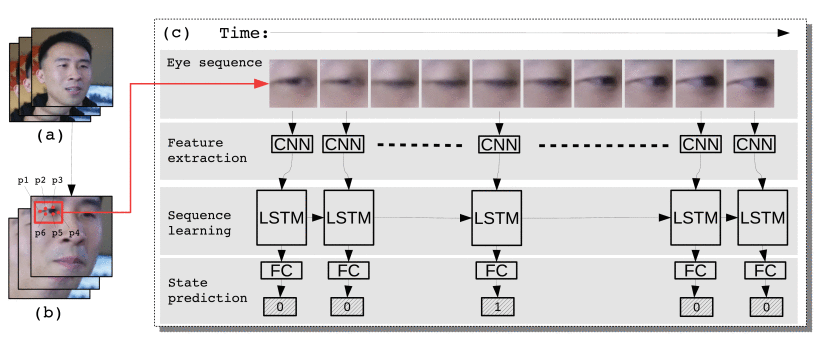
\includegraphics[width=0.75\linewidth]{images/LRCN.png}}
    \caption{Overview of the LRCN method. (a) is the original sequence. (b) is the sequence after face alignment. We crop out eye region of each frame based on eye landmarks $p_1-6$ in (b) and pass it to (c) LRCN, which consists of three parts: feature extraction, sequence learning and state prediction\cite{ictuoculi}}
    \label{fig:LRCN}
\end{figure}

The first part is a typical Convolution Neural Network (CNN) used to extract the discriminative features from the eye region. The next stage is to use a Recursive Neural Network with Long Short Term cells (LSTM-RNN) to guess the probability of eye being in range $[0,1]$ with $0$ equating to eye being open, and $1$ being eye is closed. To do this it uses the following function:

\begin{equation}
\begin{array}{l}
    f_t = \sigma \left( W_{fh} h_{t-1} + W_{fx} x_t + b _f \right) \\
    i_t = \sigma \left( W_{ih} h_{t-1} + W_{ix} x_t + b_i \right) \\
    g_t = \tanh \left( W_{ch} h_{t-1} + W_{cx} x_t + b_c \right) \\
    C_t = f_t \odot C_{t-1} + i_t \odot g_t \\
    o_t = \sigma \left( W_{oh} h_{t-1} + W_{ox} x_t + b_o \right) \\
    h_t = o_t \odot \tanh \left( C_t \right)
\end{array}
\end{equation}

$\sigma$ is the sigmoid function, $f_t$ is forget gate to control what previous memories will be discard, it is input gate to selectively pass the current input, which is manipulated by $g_t$. $o_t$ is output gate to control how much memory will be transferred into hidden state $h_t$. Memory cell $C_t$ is combined by previous memory cell $C_{t-1}$ controlled by $f_t$ and manipulated input $g_t$ controlled by $i_t$. 256 hidden units are used in the LSTM cell, which is the dimension of LSTM output $z_t$\cite{ictuoculi}. A diagram of such a cell is shown in Figure \ref{fig:LSTM}.

\begin{figure}[H]
    \centering
    \fbox{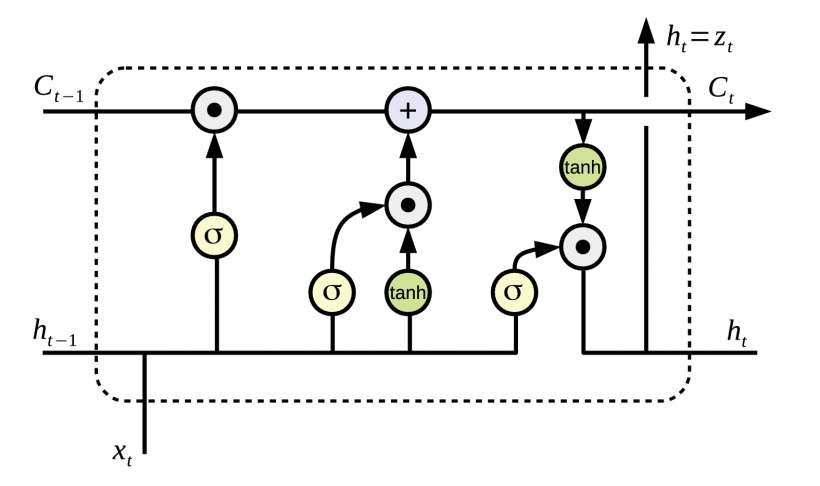
\includegraphics[width=0.5\linewidth]{images/LSTN.png}}
    \caption{A diagram of LSTM structure\cite{ictuoculi}}
    \label{fig:LSTM}
\end{figure}

Finally, the output is then used to determine whether or not a blink has occurred, and over what time period.\\

A simplified method is used to determine whether the blink patterns are consistent with a normal human being. This solely detects the number of blinks in a set period of time (60 seconds),the average person blinks 34.1 times a minute. This leads to an accuracy of 99\% when tested on a dataset of 32 videos.

\subsubsection{Analysis}

DeepVision's primary advantage is that it is very easy to compute and implement. Fast-HyperFace is a pre-trained model and therefore is a simple drag and drop implementation. Once $p_{1-6}$ are located in a frame, it is a simple calculation to determine the $EAR$. The following statistical analysis to determine if the blinking is consistent with real videos or not is also relatively simple and non-computationally intensive. Therefore any methodology involving DeepVision would be fast to implement and relatively easy to debug.\\

The primary downsides to DeepVision is potential obstruction of the eyes. $EAR$ requires the entire eye to be visible in the frame of a video to identify all of the points required. A partial $EAR$ can be calculated with a single eye but the accuracy of this is going to be less than if two eyes were visible. The second disadvantage is the database required to determine whether blinking is consistent with normal blinking. The database requires a large number of labelled examples which would be time consuming to produce.\\

Ictu Oculi has a much more complex blink-detection system, requiring two separate machine learning models to be trained to identify if a blink is happening or not. This is a lot more complex and requires pre-processing resulting in a longer development time and training time. On the other hand, it results in a much more resilient blink detection mechanism as the eyes can be partially obscured in a frame but the eye's state can still be accurately determined.\\

The drawback is that the state of the eye is binary open or close, any information relating to the speed of the blink is lost resulting in a very rudimentary system to determine whether a sequence of blinks is a DeepFake or not. This seems to have little to no effect on accuracy of detection.\\

The planned implementation can be found in Section \ref{sec:future-blink}.

\subsection{Adversarial Noise}

It has been demonstrated by various works that the majority of current DeepFake detectors, even state of the art ones, can be fooled by a variety of adversarial attacks\cite{juefei2022countering}. These work by manipulating the image produced by a DeepFake to try and throw off any detectors.

\subsubsection{Adversarial Perturbations}

The first way to try and fool DeepFakes is Fast Gradient Sign Method (FGSM)\cite{pertubations}.

\begin{equation}
    \mathbf{x}_{adv} = \mathbf{x} + \varepsilon \operatorname{sign} (\nabla _x J( \mathbf{x},\mathbf{y}, \theta ))
\end{equation}

$\mathbf{x}_{adv}$ is the image produced once the adversarial attack has been completed. $\mathbf{x}$ denotes a vector of pixel value to denote the image produced by a GAN. $J$ is the training loss function (one possible example is categorical cross-entropy loss) which takes $\theta$ as the parameters of the model. Finally $\varepsilon$, is a hyperparamter for the magnitude of perturbation per pixel. A high $\varepsilon$ leads to higher chance to disrupt the model but a higher chance the perturbations become visible to humans, it is recommended to keep $\varepsilon$ in the range [0,01, 0.1]. 0.02 was used in the paper\cite{pertubations}. Through the loss function, this will alter a pixel to the maximum allowed by $\varepsilon$ which will subtly alter each pixel enough to throw off a DeepFake detector.\\

The other method proposed by \cite{pertubations} is Carlini and Wagner $L_2$ Norm Attack ($CW-L_2$). The following method is based on the original paper\cite{carlini2017towards} and a PyTorch implementation\cite{cwl2python}. The first aim is to minimise the $L_2$ norm for the adversarial image $\mathbf{x}'$:

\begin{equation}
\label{eq:l2_norm}
    \mathop {\min} \limits_{x'} \left\{ \left\| \mathbf{x}' - \mathbf{x} \right\|_2^2 \right\}
\end{equation}

The other objective is:

\begin{equation}
\label{eq:min_f(x')}
\begin{array}{c} 
    \mathop {\min} \limits_{x'} \left\{ f\left( \mathbf{x}' \right) \right\} \\
    \text{where } f\left( \mathbf{x}' \right) = \max \left( \max_{i \ne y} \left\{ \mathbf{Z} \left( \mathbf{x}' \right)_y - \mathbf{Z} \left( \mathbf{x}' \right)_i \right\}, - \kappa \right)
\end{array}
\end{equation}

Where $\mathbf{Z}(\mathbf{x}')$ is the product of DeepFake detector. $i$ is the index of the current target class and $y$ is the index of the true target class (if no perturbations were made). Thus by minimising $f(\mathbf{x}')$, the difference between the incorrect class ($\mathbf{Z}{{\left( {{\mathbf{x}}'} \right)}_i}$) and the correct class (${\mathbf{Z}}{{\left( {{\mathbf{x}}'} \right)}_y}$) is maximised meaning a miss-classification is most likely. $\kappa$ defines a threshold for the maximum difference between the incorrect and correct classes.\\

To ensure a pixel is only floating between 0 and 1:

\begin{equation}
\label{eq:tanh}
    \mathbf{x}' = \frac{1}{2}(\tanh (\omega ) + 1)
\end{equation}

Thus combining \ref{eq:l2_norm}, \ref{eq:min_f(x')}, and \ref{eq:tanh}:

\begin{equation}
\begin{array}{c}
    \omega^\ast = \arg \min_\omega \left\{ \left\| \mathbf{x}' - \mathbf{x} \right\|_2^2 + cf\left( \mathbf{x}' \right) \right\} \\
    \mathbf{x}_{adv} = \frac{1}{2}\left( \tanh \left( \omega^\ast \right) + 1 \right)
\end{array}
\end{equation}

$c$ is a positive parameter designed to weight the two objectives of the $CS-L_2$ attack. It is typically found via binary search during run time. To determine the parameters takes a long time, however sometimes leads to better results, especially on whitebox testing:

\begin{figure}[H]
    \centering
    \fbox{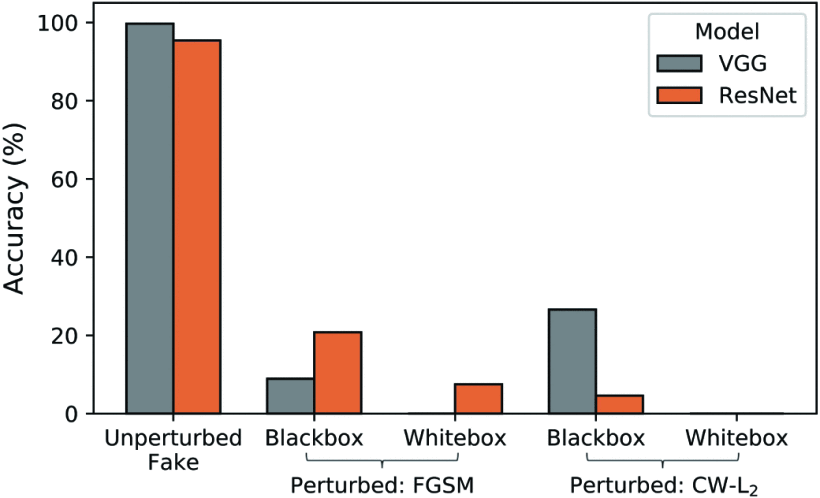
\includegraphics[width=0.5\linewidth]{images/fgsm.png}}
    \caption{Evaluation of FGSM and $CW-L_2$}
    \label{fig:fgsm}
\end{figure}

\subsubsection{FakeRetouch}

FakeRetouch is another method of adding noise to an image, using a combination of additive noise and deep image filtering to reduce artifact patterns in both the spacial and frequency domains\cite{huang2020fakeretouch}. The method uses the following equation to produce the doctored image $\hat{\mathbf{I}}$:

\begin{equation}
\begin{array}{c}
    \hat{\mathbf{I}}=\text{DNN}(\mathbf{I})\circledast (\mathbf{I} +\mathbf{A}\odot \mathbf{N}_{\sigma}) \\
    \text{where }\mathbf{A}=\arg \max _{\mathbf{A}}J(D(\mathbf{I}+\mathbf{A}), y) +||\mathbf{A}||_1
\end{array}
\end{equation}

$DNN(\mathbf{I})$ is a UNet-like neural network using kernels of $\mathbf{I}$. When combined with $\circledast$ (pixel-wise filtering), the following method can be done: for the $p$-th pixel in an image $\mathbf{I}$, is altered by the corresponding $p$-th kernel in $\mathbf{K}$ denoted as $\textbf{K}_p \in \mathbb{R}^{K \times K}$ with $k$ being the kernel size \cite{huang2020fakeretouch}. $J(\cdot)$ is a cross-entropy loss function with $y$ as the ground-truth value. $D(\cdot)$ is the DeepFake detection model being targeted. Adding the $L_1$-norm ($||A||_1$) encourages the noise to be sparse to avoid human perception of the noise. Finally, $\odot \mathbf{N}_\sigma$ adds Gaussian Noise filter with standard deviation $\sigma$. \\

The result of this method caused a drop in accuracy of detecting fake images from 88.99\% to 21.64\%. As $DNN(\mathbf{I})$ can be computed offline and then applied to every frame in a dataset, it is overall relatively quick to run.

\subsubsection{Adversarial Patch}

Adversarial Patch is a method for confusing DeepFake detectors that adds a specially crafted ``patch" to an image to confuse classifiers\cite{brown2017adversarial}.

\begin{figure}[H]
    \centering
    \fbox{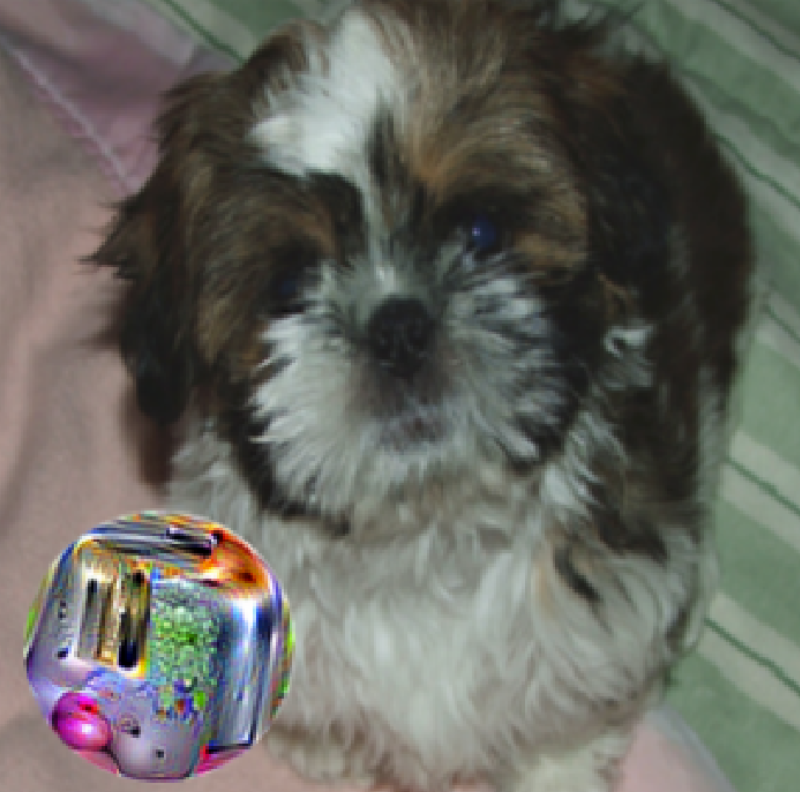
\includegraphics[width=0.25\linewidth]{images/adverserial_patch.png}}
    \caption{An image of a dog with the adversarial patch added in the bottom left\cite{brown2017adversarial}}
\end{figure}

This methodology will not be used as it is clear to a human that there is something malicious going on with the patch, even if it is not immediately obvious it would be for.

\subsubsection{Analysis}

Out of the three methods, FakeRetouch seems to be the quickest and easiest to implement. It also is the quickest to apply as there are no hyperparamters to be fine-tuned\cite{huang2020fakeretouch}. This is major factor as the model will need to be run on all the videos in the dataset to try, which could millions, possibly billions of frames, thus efficiency is key. It has slightly worse reported effectiveness than $CW-L_2$ and FGSM but this is made up for by its speed.\\

To improve testing results, a second model will also be used. This will be $CW-L_2$ as it is more effective at fooling current DeepFake detectors than FGSM (Figure \ref{fig:fgsm}). It also benefits from a pre-built PyTorch implementation \cite{cwl2python} meaning it can be used for an initial proof-of concept.\\

The planned implementation can be found in Section \ref{sec:future-noise}

\subsection{Datasets}

There is an extensive range of DeepFake datasets due to their potential to produce misinformation and other damaging content. One such example is FaceForensics++\cite{roessler2019faceforensicspp}, a vast (approximately 2TB) dataset of short clips generated through a variety of generation methods. Once you get access, you also get access to Google's \& JigSaw's DeepFake Detection Dataset\cite{DDD_GoogleJigSaw2019} which contains a (slightly smaller) set of videos.\\

Meta have also created a detection dataset\cite{DFDC2020}, made available through Kaggle\cite{kagglemeta}. This dataset contains 124,000 videos created by 8 different DeepFake generators to create a comprehensive dataset.\\

An analysis on how these datasets will be stored can be found in Section \ref{sec:datasets}

\section{Current Progress}

\subsection{Delay}

Unfortunately, the project is currently delayed by approximately 2 weeks. This is due to two primary reasons: courseworks and extent of research required.

\subsubsection{Courseworks}

In the specification, it was stated: ``whilst other modules have their coursework at the same time as this project is happening, with effective time management, there will be no major clash with timings; at least not enough to delay the course of the project significantly." It turns out some of the courseworks were more work than anticipated, most notably compilers. This lead to the project being delayed by roughly two weeks.\\

To remedy this, Wednesday afternoons have been set aside as dedicated time to work on project. Other times will also be used should there be any free time available. Additionally, next term, there are fewer modules being taken which will have smaller courseworks and thus the workload that is not project related will be reduced.

\subsubsection{Research Required}

The initial project specification called was written assuming that the project would only be implementing an existing DeepFake detection methodology that only existed as a theoretical proof of concept. The chosen methodology, blink detection, involves two models: one to determine the state of the eyes, and the other to determine whether the sequence produced by the previous model is feasible. Additionally, methods to add adversarial noise to image needed to be researched. Thus the research phase took three weeks rather than the intended two, further setting the project behind.

\subsection{Literature Review}

The majority of progress made on this project has been the literature review as detailed in Section \ref{sec:literature-review}. This involved researching the various aspects of the field and seeing what existing research. For example, for blink detection, comparing DeepVision versus Ictu Oculi.\\

After reviewing the variable literature, they were analysed to work out which approach would be most appropriate in this scenario given: time, difficulty, and effectiveness. Once the various methods were evaluated, a proposal for both a proof of concept and the final version were made. This plan will then be implemented in due course as laid out in Section \ref{sec:future-progress}.

\subsection{Datasets} \label{sec:datasets}

Obviously, DeepFake detection datasets are incredibly large and so there is a difficulty in how they can be stored. The typical maximal allowance of an account on the department of computer science's systems is 500GB (an increase from 25GB)\cite{dcsquota}. The department has been contacted about the viability of storing such a large amount of data (approximately 10TB once images have been updated with a noise masks). Possible solutions are: to use old hard drives and attach them to the existing computer science compute cluster; use the  Scientific Computing Research Technology Platform (SCRTP) clusters which has the appropriate specifications to handle large volumes of data; or to only test partial amounts of each dataset at a time. An account has been requested with SCRTP.\\

To gain access to most of the datasets, a Google form has to be filled in to prove and confirm that you will only use the dataset for academic purposes. Such forms for all relevant datasets have been filled out. As of writing (18th November), permission has been granted to access FaceForensics++ and Google's DeepFake Detection Dataset.

\section{Future Progress} \label{sec:future-progress}
\subsection{Proof of Concept}

Over the Christmas holiday, to test if all the research presented previously is valid, a proof of concept of both the blink detection mechanism and adversarial noise injector will be made. These are intended to be quick and so will use pre-trained models and existing codebases, such as Google's MediaPipe\cite{mediapipe}. 

\subsection{Blink Detection} \label{sec:future-blink}

The primary disadvantage of the $EAR$ is that it cannot calculate the state of an eye if any of $p_{1-6}$ is obscured\cite{ictuoculi}. However, various AI models such as Google's MediaPipe \cite{mediapipe} and OpenFace\cite{openface} maintain detection of these features even when obscured. Hence it is possible to maintain an accurate $EAR$ even when the face is partially obscured in a frame. Therefore, for the blink detection in my project, I will initially use MediaPipe as a proof of concept and then move on to training my own model from various eye datasets such as Kaggle's eye blinking prediction\cite{eyeblinkprediction}.\\

Having the $EAR$ data allows for more sophisticated methods of blink detection than what was utilised than Ictu Oculi. However a method such as the database employed by DeepVision\cite{blinking-pattern} would be too time consuming to label and store all the data given the amount of time given to this project. Given the large amount of data available: such as the time taken to blink, the period between blinking, and the overall progression of the $EAR$ it may be possible to train a classifier neural network to determine whether or not a sequence of $EAR$ readings overtime is a that of a genuine video or a DeepFake. As this has never been done before, further research and experimentation would need to be done. For a proof of concept, Ictu Oculi has proved even a simple approach of frequency of blinks is sufficient\cite{ictuoculi}.

\subsection{Adversarial Noise} \label{sec:future-noise}

Because there is a pre-existing implementation\cite{cwl2python}, when developing a proof-of-concept, $CW-L_2$ will be used as the method to add noise to a subset of images. All methods of adversarial noise injection require the model being targeted to be fully developed, therefore this has to be trained after the blink detection model is trained.\\

Once a proof of concept has been verified and the full blink detector is trained, a full version of FakeRetouch and $CW-L_2$ shall be trained to act as a testing dataset when evaluating how resilient a blink-based DeepFake detector is.

\subsection{Timeline} \label{sec:timeline}

{\huge INSERT GANTT CHART HERE}

\section{Appraisals \& Reflections}

Overall progress has been slower than expected, even given the unforeseeable delays. Obviously I am disappointing with this as it means more work in the future. However, given the plan defined in Section \ref{sec:timeline} has clear steps and finishing points, I am confidence that the future progress of this dissertation will be consistent.\\

On the other hand, the development of my research skills is welcome. Until now, I had not undertaken a significant amount of academic research at any kind of scale. For example, this is the first time I have ever used Google Scholar. Completing the literature review has shown me that research is something that I can do which I am grateful for.

\section{Legal, Social, Ethical, and Professional Issues \& Considerations}

The only valid consideration with this project is the use of datasets that are covered by licenses. This is covered by declaring the intended manipulation of the data when requesting access via the various Google forms.\\

There are no further legal, social, ethical, and professional issues \& considerations.

\section{Project Management}

The code for this project is spread out over various platforms: initial development on the DCS systems; large scale compute on either the DCS or SCRTP HPC clusters; and finally report development in Overleaf. Therefore it will be crucial to centrally track all code to avoid loosing track of changes made. The central tracker will be a git repository stored in the cloud via GitHub. To avoid overloading individual systems, certain parts of the repository will not be tracked enabled by \verb|.gitignore|. An obvious example is the datasets themselves which will only be stored on the the HPC clusters.\\

GitHub can also be used to keep track of current progress through the use of the issues and tasks tab. Each issue can have multiple tasks assigned to it, only when all tasks have been completed can the issue be marked as ``completed". This can then effectively track progress throughout the project.\\

The central repository for this project can be found at \url{https://github.com/Mole1424/3rd-year-project}.\\

To monitor progress, regular meetings with my supervisor will be taken to ensure the work is being done.\\

\bibliographystyle{IEEEtran}
\bibliography{progress}

\newpage
\appendix
\import{spec/}{spec.tex}

\end{document}